\documentclass[12pt]{report}

\usepackage{blindtext} %%%Temporary package for gibberish
%%%%%%%%%%%%%%%%%%%%%%%%%%%%%%%%%%%%%%%%%%%%%%%%%%%%%%%%
%%%%%%%%%%%%%%%%%%%%%packages%%%%%%%%%%%%%%%%%%%%%%%%%%%
%%%%%%%%%%%%%%%%%%%%%%%%%%%%%%%%%%%%%%%%%%%%%%%%%%%%%%%%
\usepackage{fancyhdr} %header package
\usepackage[margin=1in,tmargin=0.85in,headsep=0.2in]{geometry}
\usepackage{anyfontsize}
\usepackage{background}
\usepackage{fontspec}
\usepackage{graphicx}
\usepackage{lastpage}
\usepackage[absolute,overlay]{textpos}
\usepackage[explicit]{titlesec}
\usepackage{setspace}
\usepackage{etoolbox}
\usepackage{chngcntr}
\usepackage{nameref} % Used to reference chapter/section names vice number
\usepackage{tocloft}
\usepackage{caption}
\usepackage{natbib}
\usepackage{hyperref}
\usepackage{paralist}
\usepackage[acronyms,toc,nomain,automake]{glossaries} % Acronym glossary
\usepackage{pdfpages} %used to input whole pdf pages: final page
\usepackage{appendix}
\usepackage{nicefrac}
%\usepackage{gensymb}
\usepackage{silence} %silences deprecated warnings for format
\usepackage{amsthm}
\usepackage{amsmath}
\usepackage{float} %helps place figures/tables
%%%%%%%%%%%%%%%%%%%%%%%%%%%%%%%%%%%%%%%%%%%%%%%%%%%%%%%%
%%%%%%%%%%%%%%%%%%%%%%%%%%%%%%%%%%%%%%%%%%%%%%%%%%%%%%%%

%%%%%%%%%%%%%%%%%%%%%%%%%
%%%% TITLE VARIABLES %%%%
%%%%%%%%%%%%%%%%%%%%%%%%%
\newcommand{\reportno}{REPORT NO:  USNTPS/RTR-2019/01}
\newcommand{\header}{USNTPS/RTR-2019/01}
\newcommand{\rpttitle}{REPORT TITLE}
\newcommand{\name}{RANK First Last, SERVICE}
\newcommand{\rptdate}{DD Month YYYY}
%%%%%%%%%%%%%%%%%%%%%%%
%%%%%%%%%%%%%%%%%%%%%%%
%%%%%%%%%%%%%%%%%%%%%%%

%%%%%%%%%%%%%%
%%%% misc %%%%
%%%%%%%%%%%%%%
\makeglossaries
\WarningFilter{glossaries}{Deprecated command}% Removes warning starting with "Deprecated command"
\counterwithout{figure}{chapter} %starts figure counting from 1. Independent of location within chapter/section.
\counterwithout{table}{chapter} %starts table counting from 1. Independent of location within chapter/section.
\renewcommand{\headrulewidth}{0pt} %removes header underline
\backgroundsetup{contents={}} %sets background image ("watermark")
\doublespacing
\setmainfont{Times New Roman}
\makeatletter
\patchcmd{\chapter}{\if@openright\cleardoublepage\else\clearpage\fi}{}{}{} %modifies \chapter so that it doesn't clear page automatically
\makeatother
% initial header/footer setup
\fancypagestyle{plain}
{%  the preset of fancyhdr 
    \fancyhf{} % clear all header and footer fields
    \fancyfoot[C]{\thepage} % except the center
    \fancyhead[L]{\header}
    \renewcommand{\headrulewidth}{0pt}
    \renewcommand{\footrulewidth}{0pt}}
\pagestyle{fancy}

\DeclareCaptionType{afigure}[Figure][] % Create appendix figure environment
\DeclareCaptionType{atable}[Table][] % Creates appendix table environment
\renewcommand{\bibname}{References} % Change title of bibliography to References
\makeatletter
\renewcommand\@biblabel[1]{#1.} % Change style of bibliography to list reference with a number followed by a period. E.g., 1.
\makeatother
\setcitestyle{numbers} % Sets citation style to numerical. Use \citenum{} to not get parentheses
% Change the appendix figure/table caption style to A-1, B-1 from A.1
\renewcommand{\theafigure}{\thechapter-\arabic{afigure}}
\renewcommand{\theatable}{\thechapter-\arabic{atable}}
%Change equation style for tags
\renewcommand{\theequation}{\textit{Eqn} \arabic{equation}} 

%Marcos page formatting below
% Header and footer format
\fancyhf{}
\fancyhead[L]{\header}
\fancyfoot[C]{\thepage}
\setlength{\voffset}{0in}
\setlength{\headheight}{14.5pt}
\setlength\parindent{0cm}

%Paragraph formatting and counting
\newcommand{\parnum}{\arabic{parcount}.}
\newcommand{\pp}{\newline \vspace{-2ex}}
\newcounter{parcount}
\newcommand\p{%
    \refstepcounter{parcount}%
    \parnum \hspace{0.5em}%
}
\renewcommand{\headrulewidth}{0pt}
\renewcommand{\footrulewidth}{0pt}
\titleformat
{\chapter} % command
[hang] % shape
{} % format
{} % label
{0ex} % sep
{\centering\MakeUppercase{#1}} % before-code
[] % after-code
\titlespacing{\chapter}{0ex}{0ex}{3ex}

\titleformat
{\section} % command
[hang] % shape
{} % format
{} % label
{0ex} % sep
{\MakeUppercase{\underline{#1}}} % before-code
[] % after-code
\titlespacing{\section}{0ex}{0ex}{0.5ex}

\titleformat
{\subsection} % command
[hang] % shape
{} % format
{} % label
{0ex} % sep
{\MakeUppercase{#1}} % before-code
[] % after-code
\titlespacing{\subsection}{0ex}{0ex}{-1ex}

\titleformat
{\subsubsection} % command
[hang] % shape
{} % format
{} % label
{0ex} % sep
{\underline{#1}} % before-code
[] % after-code
\titlespacing{\subsubsection}{0ex}{0ex}{-1ex}
%%%%%%%%%%%%
%%%%%%%%%%%%
%%%%%%%%%%%%

%%%%%%%%%%%%%%%% Table of Contents formatting %%%%%%%%%%%%%%%%%%%%%
%%%%%%%%%%%%%%%%%%%%%%%%%%%%%%%%%%%%%%%%%%%%%%%%%%%%%%%%%%%%%%%%%%%
\setcounter{tocdepth}{2}
\renewcommand{\cftchapdotsep}{2} %change dot spacing/step/density
\renewcommand{\cftsecdotsep}{2}
\renewcommand{\cftsubsecdotsep}{2}
\renewcommand{\cftfigdotsep}{2}
\renewcommand{\cfttabdotsep}{2}
\renewcommand\numberline[1]{} %remove chap/sec numbering from TOC
\renewcommand{\cftchapfont}{\normalfont}
\renewcommand\cftchappagefont{\normalsize} %unbold page numbers
\setlength{\cftbeforetoctitleskip}{0em} %move TOC title up or down
\renewcommand{\cfttoctitlefont}{\hfil \normalfont\normalsize} %set TOC font and size
\renewcommand{\cftloftitlefont}{\hfil \normalfont\normalsize}
\renewcommand{\cftlottitlefont}{\hfil \normalfont\normalsize}
\addtocontents{toc}{~\hfill\normalfont\underline{Page No.}\par} %place "_Page No._" over page numbers
%Add page number on top of the list of figures with added vertical space
\addtocontents{lof}{~\hfill\normalfont\underline{Page No.}{\vspace{10pt}}\par}
\addtocontents{lot}{~\hfill\normalfont\underline{Page No.}{\vspace{10pt}}\par}
\renewcommand*\listfigurename{Figures} %name LOF
\renewcommand*\listtablename{Tables}
\setlength{\cftfigindent}{0pt} %force zero indent of LOF to match TOC
\setlength{\cfttabindent}{0pt}
\cftsetindents{section}{0.25in}{0.5in} %set indents in TOC
\cftsetindents{subsection}{0.5in}{0.5in}
\cftsetindents{subsubsection}{0.75in}{0.5in}
\setlength\cftaftertoctitleskip{0pt} %set spacing between TOC title and TOC content
\setlength\cftafterloftitleskip{0pt}
\setlength\cftafterlottitleskip{0pt}
\renewcommand{\cftchapleader}{\normalfont\cftdotfill{\cftsecdotsep}}% Unbold dots for chapters
\addtocontents{loafigure}{~\hfill\normalfont\underline{Page No.}\par}
\addtocontents{loatable}{~\hfill\normalfont\underline{Page No.}\par}
% Commands to remove space between chapters in the list of figures/list of tables
\newcommand*{\noaddvspace}{\renewcommand*{\addvspace}[1]{}}
\addtocontents{lot}{\protect\noaddvspace}
\addtocontents{lof}{\protect\noaddvspace}
%%%%%%%%%%%%%%%%%%%%%%%%%%%%%%%%%%%%%%%%%%%%%%%%%%%%%%%%%%%%%%%%%%%
%%%%%%%%%%%%%%%%%%%%%%%%%%%%%%%%%%%%%%%%%%%%%%%%%%%%%%%%%%%%%%%%%%%

\begin{document}

\begin{titlepage} % ensure you have a clean path to graphics folder

\begin{picture}(50,50) %calls static background image, sets reservation of rectangular space in document for image (50x50pt)
\put(-80,-690){\hbox{
\includegraphics[scale=1.02]{graphics/title_pg1}}} %places object with start point (x, y}
\end{picture}

\vspace*{2.6cm} %sets vertical spacing offset from LaTeX's desired positioning
\hspace*{-1.5cm} %sets horizontal spacing offset from LaTeX's desired positioning
\fontsize{12}{12}\selectfont \reportno{}

\begin{center} %center text horizontally
\vspace*{5.cm}
\fontsize{14}{12}\selectfont \bfseries {\rpttitle{}}
\end{center}

\begin{center}
\fontsize{12}{12}\selectfont {by}
\end{center}

\begin{center}
\fontsize{12}{12}\selectfont {\name{}}
\end{center}

\begin{center}
\vspace*{1.cm}
\fontsize{12}{12}\selectfont {\rptdate}
\end{center}

\end{titlepage}

\pagebreak
\pagenumbering{roman}

\chapter{Summary}

\setlength{\parindent}{7ex}
“Exploration is in our nature. We began as wanderers, and we are wanderers still. We have lingered long enough on the shores of the cosmic ocean. We are ready at last to set sail for the stars.”

Testing reference... UH-60 TM, reference \citenum{UH60}.

\pagebreak

\pagebreak
\singlespacing
\vspace*{-.5cm}
\tableofcontents\newpage
\addcontentsline{toc}{chapter}{Figures}
\vspace*{-2.2cm}

\renewcommand\numberline[1]{\hbox to 24pt{#1.}} % Add numbers to list of figures and tables. The Word example doesn't add numbers, but the Test Reporting Handbook does. Including this here in case we want numbers. Delete line if we do not.

\listoffigures

\addcontentsline{toc}{chapter}{Tables}
\vspace*{-.5cm}
\listoftables\newpage

\doublespacing
\setlength\parindent{0cm} % Added to eliminate indented, numbered paragraphs
\pagenumbering{arabic}

\chapter{Introduction}\label{ch:Introduction}

%NEW SECTION
\section{Background}\label{sec:Background}
\p \blindtext \pp \label{par:Background}

%NEW SECTION
\section{Purpose}\label{sec:Purpose}
\p \blindtext \pp \label{par:Purpose}

%NEW SECTION
\section{Description of Test Aircraft}\label{sec:Description}

\subsection{Basic Aircraft}\label{subsec:Aircraft}
\p Text \pp \label{par:BasicAircraft}

\subsection{Test Aircraft Modifications}\label{subsec:TestAircraft}
\p Text \pp \label{par:TestAircraft}

%NEW SECTION
\section{Scope of Test}\label{sec:Scope}
\subsection{Test Envelope and Flight Clearance}\label{subsec:TestEnvelope}
\p Text \pp \label{par:TestEnvelope}

\subsection{Test and Test Conditions}\label{subsec:TestConditions}
\p Text \pp \label{par:TestConditions}

\subsection{Test Criteria}\label{subsec:TestCriteria}
\p Text \pp \label{par:TestCriteria}

%NEW SECTION
\section{Method of Test}\label{sec:MethodTest}
\p Text \pp \label{par:MethodTest}

%NEW SECTION
\section{Chronology}\label{sec:Chronology}
\p Text \pp \label{par:Chronology}

\pagebreak


\chapter{Results and Evaluation}\label{ch:RandE}

%NEW SECTION
\section{Mission Suitability}\label{sec:MissionSuitability}
\subsection{Air to Air}\label{subsec:airtoair}
\p It's pretty ok. \pp \label{par:airtoair}

\subsection{Air to Ground}\label{subsec:airtoground}
\p Kinda decent. \pp \label{par:airtoground}

%NEW SECTION
\section{Mission Tasks}\label{sec:MissionTasks}
\subsection{Take-Off}\label{subsec:takeoff}
\p It does it. \pp \label{par:takeoff}

\subsection{Landing}\label{subsec:landing}
\p Does this too. \pp \label{par:landing}

%NEW SECTION
\section{Test Article Characteristics}\label{sec:TestArticle}
\subsection{Speed}\label{subsec:speed}
\p Flies fast, flies slow. \pp \label{par:speed}

\subsection{Maneuverability}\label{subsec:maneuverability}
\p Brings all the boys to the yard. \pp \label{par:manueverability}

\pagebreak

\chapter{Supporting Data}\label{ch:Data}

%NEW SECTION
\section{General}\label{sec:SupportingGeneral}
\p Check out figure \ref{fig:my_label1} \pp \label{par:SupportingGeneral}

\begin{figure}[htb]
    \centering
    
\includegraphics[width=0.4\columnwidth]{figures/usntps.png}
    \caption{United States Naval Test Pilot School Emblem}
    \label{fig:my_label1}
\end{figure}

\pagebreak

%NEW SECTION
\section{Mechanical Characteristics}\label{sec:MechChar}
\p Pick a lucky number in table \ref{tab:my_label2} \pp \label{par:MechChar}

\begin{table}[htb]
    \caption{Table of Random Numbers}
    \label{tab:my_label2}    
    \centering
    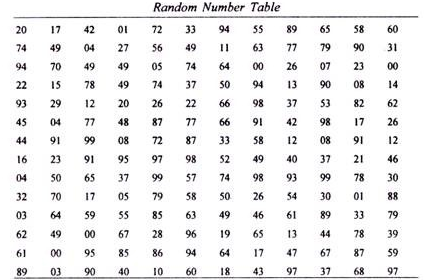
\includegraphics{tables/table.png}
\end{table}

\pagebreak

\chapter{Conclusions}\label{ch:Conclusion}

%NEW SECTION
\section{General}\label{sec:ConclusionGeneral}
\p The F-18 aircraft is satisfactory for the air to air mission. \pp \label{par:ConclusionGeneral}

%NEW SECTION
\section{Enhancing Characteristic}\label{sec:Enhancing}
\p Flying around is cool (paragraph \ref{par:ConclusionGeneral}) \pp \label{par:Enhancing_1}

%NEW SECTION
\section{Part I Deficiency}\label{sec:ConclusionsPartI}
\p Canted pylons are the dumbest shit ever. \pp \label{par:Conc_partI_1}

%NEW SECTION
\section{Part II Deficiencies}\label{sec:ConclusionsPartII}
\p This was annoying. \pp \label{par:Conc_partII_1}

\p This was also annoying. \pp \label{par:Conc_partII_2}

%NEW SECTION
\section{Part III Deficiencies}\label{sec:ConclusionsPartIII}
\p This could be done without. \pp \label{par:Conc_partIII_1}

\p This could be done without. \pp \label{par:Conc_partIII_2}

%NEW SECTION
\section{Specification Compliance}\label{sec:SpecCompliance}
\p It met some of the requirements, probably. \pp \label{par:Spec_comp_1}

\pagebreak

\chapter{Recommendations}\label{ch:Recommend}

%NEW SECTION
\section{General}\label{sec:RecGeneral}
\p Include the enhancing characteristic in \pp

\p Correct the Part I deficiency in paragraph \ref{par:TestCriteria} when possible. \pp

\p Correct the Part II deficiencies in paragraphs xx as soon as practicable. \pp

\p Avoid the Part III deficiencies in paragraphs x and x in future designs. \pp

%NEW SECTION
\section{Specific}\label{sec:RecSpecific}
\p Consideration should be given to making a better aircraft. \pp

\clearpage
\addcontentsline{toc}{chapter}{References}
\bibliography{TPS}
\bibliographystyle{abbrvnat}

%\usepackage[acronyms,nomain,toc,automake]{glossaries} %this is the proper preamble command
%\makeglossaries also required in preamble

\label{Acronyms}

%============== Your acronyms here! ================%
% \newacronym{reference}{Displayed}{Long description}

\newacronym{ufc}{UFC}{Up Front Control}
\newacronym{acm}{ACM}{Air Combat Manuevering}
\newacronym{lol}{LOL}{laugh out loud}
\newacronym{as}{A/S}{Air to Surface}

% by default this will only print acronyms used in the document, this command will display all acronyms added in this file
\glsaddall[types=\acronymtype]

\newglossarystyle{mylistdotted}{\glossarystyle{listdotted}%
   \renewenvironment{theglossary}{\begin{compactdesc}}{\end{compactdesc}}%
   \renewcommand*{\glsgroupskip}{}}

\begin{singlespacing}
\printglossary[title={Acronyms and Abbreviations},type=\acronymtype, style=mylistdotted]
\end{singlespacing}


%================== How to use this ======================================
%\gls command will display "<full> (<abbrv>)" of first use. On subsequent uses only the abbreviation will be displayed.

%To reset the first use of an acronym, use the command:

%\glsreset{<label>} or, if you want to reset the use status of all acronyms: \glsresetall 

%Similarly, to unset the first use of an acronym so that only the abbreviation will be displayed, use: %\glsunset{<label>} or, for all acronyms:  \glsunsetall

%\acrlong{ }  %Displays the phrase which the acronyms stands for. Put the label of the acronym inside the braces. In the example, \acrlong{gcd} prints Greatest Common Divisor.

%\acrshort{ }  %Prints the acronym whose label is passed as parameter. For instance, \acrshort{gcd} renders as GCD.

%\acrfull{ }  %Prints both, the acronym and its definition. In the example the output of \acrfull{lcm} is Least Common Multiple (LCM).

%%%%%%%%%%%%%%%%%%% Start of the Appendices %%%%%%%%%%%%%%%%%
\newpage
\begin{appendices}
\begin{singlespacing}
% Redefine header and footer style for the appendices
\fancypagestyle{plain}
{%  the preset of fancyhdr 
    \fancyhf{} % clear all header and footer fields
    \fancyfoot[C]{\thepage} % except the center
    \fancyhead[L]{\header}
    \fancyfoot[R]{Appendix \thechapter}
    \renewcommand{\headrulewidth}{0pt}
    \renewcommand{\footrulewidth}{0pt}}
	\pagestyle{plain}% Set page style to plain.

\chapter{Appendix \thechapter: Figures}\label{app:Figures}

\renewcommand\numberline[1]{\hbox to 62pt{Figure #1:\hspace{1ex}}} % Add numbers and text to list of figures

\vspace*{-2.5cm}
\listofafigures

\pagebreak

Testing the referencing command for this appendix... Reference Appendix \ref{app:Figures}.

Testing the reference to figure \ref{fig:tpslogo}

\begin{afigure}[htb]
    \centering
    
\includegraphics[width=0.4\columnwidth]{figures/usntps.png}
    \caption{United States Naval Test Pilot School Emblem}
    \label{fig:tpslogo}
\end{afigure}

\pagebreak


%%%%%%%%%%%%%%%%%%%%%%%%%%%%%%%%%%%%%%%%%%%%%%%%%%%
%%%%%%%%%%%%%%%%%%%%%% NOTE %%%%%%%%%%%%%%%%%%%%%%%
%%%%%%%%%%%%%%%%%%%%%%%%%%%%%%%%%%%%%%%%%%%%%%%%%%%
% 
% Use \begin{afigure} and \end{afigure} for all figures that are included in the Appendix. This is to be able to generate a seperate list of figures.
\chapter{Appendix \thechapter: Tables}\label{app:Tables}

\renewcommand\numberline[1]{\hbox to 56pt{Table #1:\hspace{1ex}}} % Add numbers and text to list of tables

\vspace*{-2.5cm}
\listofatables

\pagebreak

Testing the referencing command for this appendix... Reference Appendix \ref{app:Tables}.

\begin{atable}[htb]
    \caption{Table of Random Numbers}
    \label{tab:my_label4}
    \centering
    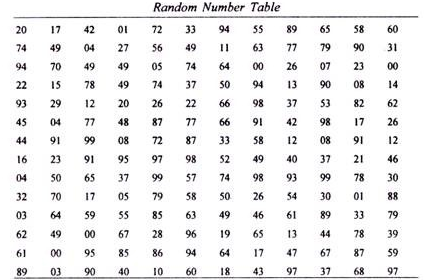
\includegraphics{tables/table.png}
\end{atable}

\newpage

\begin{atable}[htb]
    \caption{Table of Random Numbers}
    \label{tab:my_label5}    
    \centering
    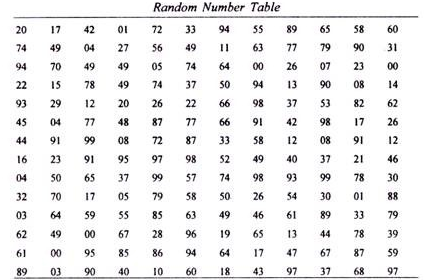
\includegraphics{tables/table.png}
\end{atable}


\pagebreak

%%%%%%%%%%%%%%%%%%%%%%%%%%%%%%%%%%%%%%%%%%%%%%%%%%%
%%%%%%%%%%%%%%%%%%%%%% NOTE %%%%%%%%%%%%%%%%%%%%%%%
%%%%%%%%%%%%%%%%%%%%%%%%%%%%%%%%%%%%%%%%%%%%%%%%%%%
% 
% Use \begin{atable} and \end{atable} for all tables that are included in the Tables Appendix section. This is to be able to generate a seperate list of tables.
\end{singlespacing}
\end{appendices}
%%%%%%%%%%%%%%%%%%%%%%%%%%%%%%%%%%%%%%%%%%%%%%%%%%%%%%%%%%%%%
\clearpage

\includepdf{graphics/final_pg.pdf}  % Final page

\end{document}